\documentclass{article}
\usepackage{gensymb, amsmath, float, graphicx, epstopdf}
\restylefloat{table}
\usepackage[margin=0.75in]{geometry}
\usepackage{verbatim}
\begin{document}

\title{Ocean Bowl Bootcamp 6: Coasts and Beaches}
\author{Michael Shen}
\maketitle

\section{Coastlines}

\begin{itemize}
	\item \textbf{Coastlines} are boundaries where the land and sea interact including both the land and water, such as bays and estuaries.
	\item The \textbf{shore} is the region where waves/tides directly affect the coastline (smashing against the surface as well as scraping the sea floor).
	\item The \textbf{beach} is an accumulation of sediment that occupies a portion of the shoreline, commonly up to the high tide levels.
	\item \textbf{Erosional} coasts primarily lose sediment, while \textbf{depositional} coasts primarily gain sediment.
	\item \textbf{Active coasts} are on an active plate boundary, while \textbf{passive coasts} are not. These are also called \textbf{active and passive margins}, respectively.
	\item Most coasts along the eastern United States are passive coasts and are considered depositional.
	\item Most coasts along the western United States are active coasts and are considered erosional.
\end{itemize}
	
\section{Types of Coasts}

\begin{itemize}
	\item \textbf{Primary coasts} are maintained mainly by geological processes. They are maintained by:
	\begin{enumerate}
		\item Erosion of the land and potential subsidence or sea level rises
		\item Sediments deposited at the shore by rivers, glaciers, or the wind (fjords, dune coasts)
		\item Volcanic activity (lava coasts and crater coasts)
		\item Vertical movements of the shoreline by tectonic processes (fault bays and fault coasts)
	\end{enumerate}
	
	\item \textbf{Secondary coasts} are maintained mainly by marine processes and were once primary coasts. They are maintained by:
	\begin{enumerate}
		\item Erosion by waves and currents (Sea arches, sea caves, and sea stacks)
		\item Dissolution by seawater (Sea arches, sea caves, and sea stacks)
		\item Deposition of sediments by waves, tides, and currents (Salt marshes)
		\item Erosion, deposition, and binding of sediments and skeletal materials by marine plants and animals (Reef coasts)
	\end{enumerate} 
	\item This classification scheme is based on the forces that shape the coasts, \textbf{not} on the age or how they appear. However, primary coasts are often younger and contain coarser sediment, while secondary coasts are often older and contain finer sediment.
\end{itemize}

	\subsection{Secondary Coasts}
	
	\begin{itemize}
		\item Eroded materials are often removed from the exposed beaches and deposited offshore. Three major types of deposits are commonly found:
		\begin{enumerate}
			\item \textbf{Bars}, which are sand deposits paralleling the shore in shallow water
			\item \textbf{Barrier islands}, which are essentially bars of sand where the sediment supply from the beach and longshore currents has been sufficient to break the surface. They protect the continental coastline from storms because they take the brunt of the damage, e.g. Galveston Hurricane
			\item \textbf{Spits and hooks}, which are bar-like deposits connected to the shoreline and often extended across the mouths of bays.  If a spit continues to build offshore and happens to connect with an offshore island, it is called a \textbf{tombolo}.
		\begin{figure}[H]
   		\centering
    		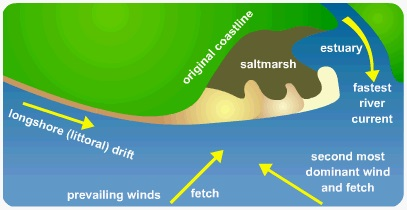
\includegraphics[scale=0.8]{./Images/BC6_Spit.jpg}
		\end{figure}
		\end{enumerate}

		\item \textbf{Reef coasts}, which form in tropical/subtropical coastal regions when plants and animals bind and trap sediment or create massive structures of their own skeletal materials. 
		\item Low-lying tidal deposits, where sedimentation and plant growth have matched subsidence and recent sea level fluctuations, create great stretches of \textbf{salt marshes}. Salt marshes are extremely productive ecosystems, and many of the world's fisheries depend on their survival.
	\end{itemize}
	
	\subsection{Beaches}
	
	\begin{itemize}
		\item The shore may be subdivided into three major regions called the \textbf{backshore, foreshore, and offshore}. The foreshore and backshore combined is a beach. \textbf{Sand bars} are often found offshore, parallel to the shore and separated by troughs.
		\begin{figure}[H]
   		\centering
    		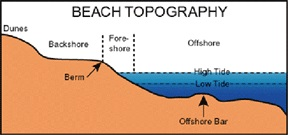
\includegraphics[scale=0.8]{./Images/BC6_BeachProfile.jpg}
		\end{figure}
		\item Some shorelines do not have visible beaches, instead they may simply have cliff faces (duh?).
	\end{itemize}
\end{document}